%%% template.tex
%%%
%%% This LaTeX source document can be used as the basis for your technical
%%% paper or abstract. Intentionally stripped of annotation, the parameters
%%% and commands should be adjusted for your particular paper - title, 
%%% author, article DOI, etc.
%%% The accompanying ``template.annotated.tex'' provides copious annotation
%%% for the commands and parameters found in the source document. (The code
%%% is identical in ``template.tex'' and ``template.annotated.tex.'')

\documentclass[conference]{acmsiggraph}

\usepackage[brazilian]{babel}
\usepackage[utf8]{inputenc}
\usepackage[T1]{fontenc}

\usepackage[font=bf]{caption}
\usepackage{subcaption}

\TOGonlineid{45678}
\TOGvolume{0}
\TOGnumber{0}
\TOGarticleDOI{1111111.2222222}
\TOGprojectURL{}
\TOGvideoURL{}
\TOGdataURL{}
\TOGcodeURL{}

\title{Paralelização da interpolação \textit{Inverse Distance Weighted (IDW)} utilizando CUDA}

\author{Andrey Rodrigues\thanks{e-mail:arodrigues@tecgraf.puc-rio.com}\\Tecgraf}
\pdfauthor{Andrey Rodrigues}

\keywords{CUDA, IDW, algorithm, shared memory}

\begin{document}

 \teaser{
 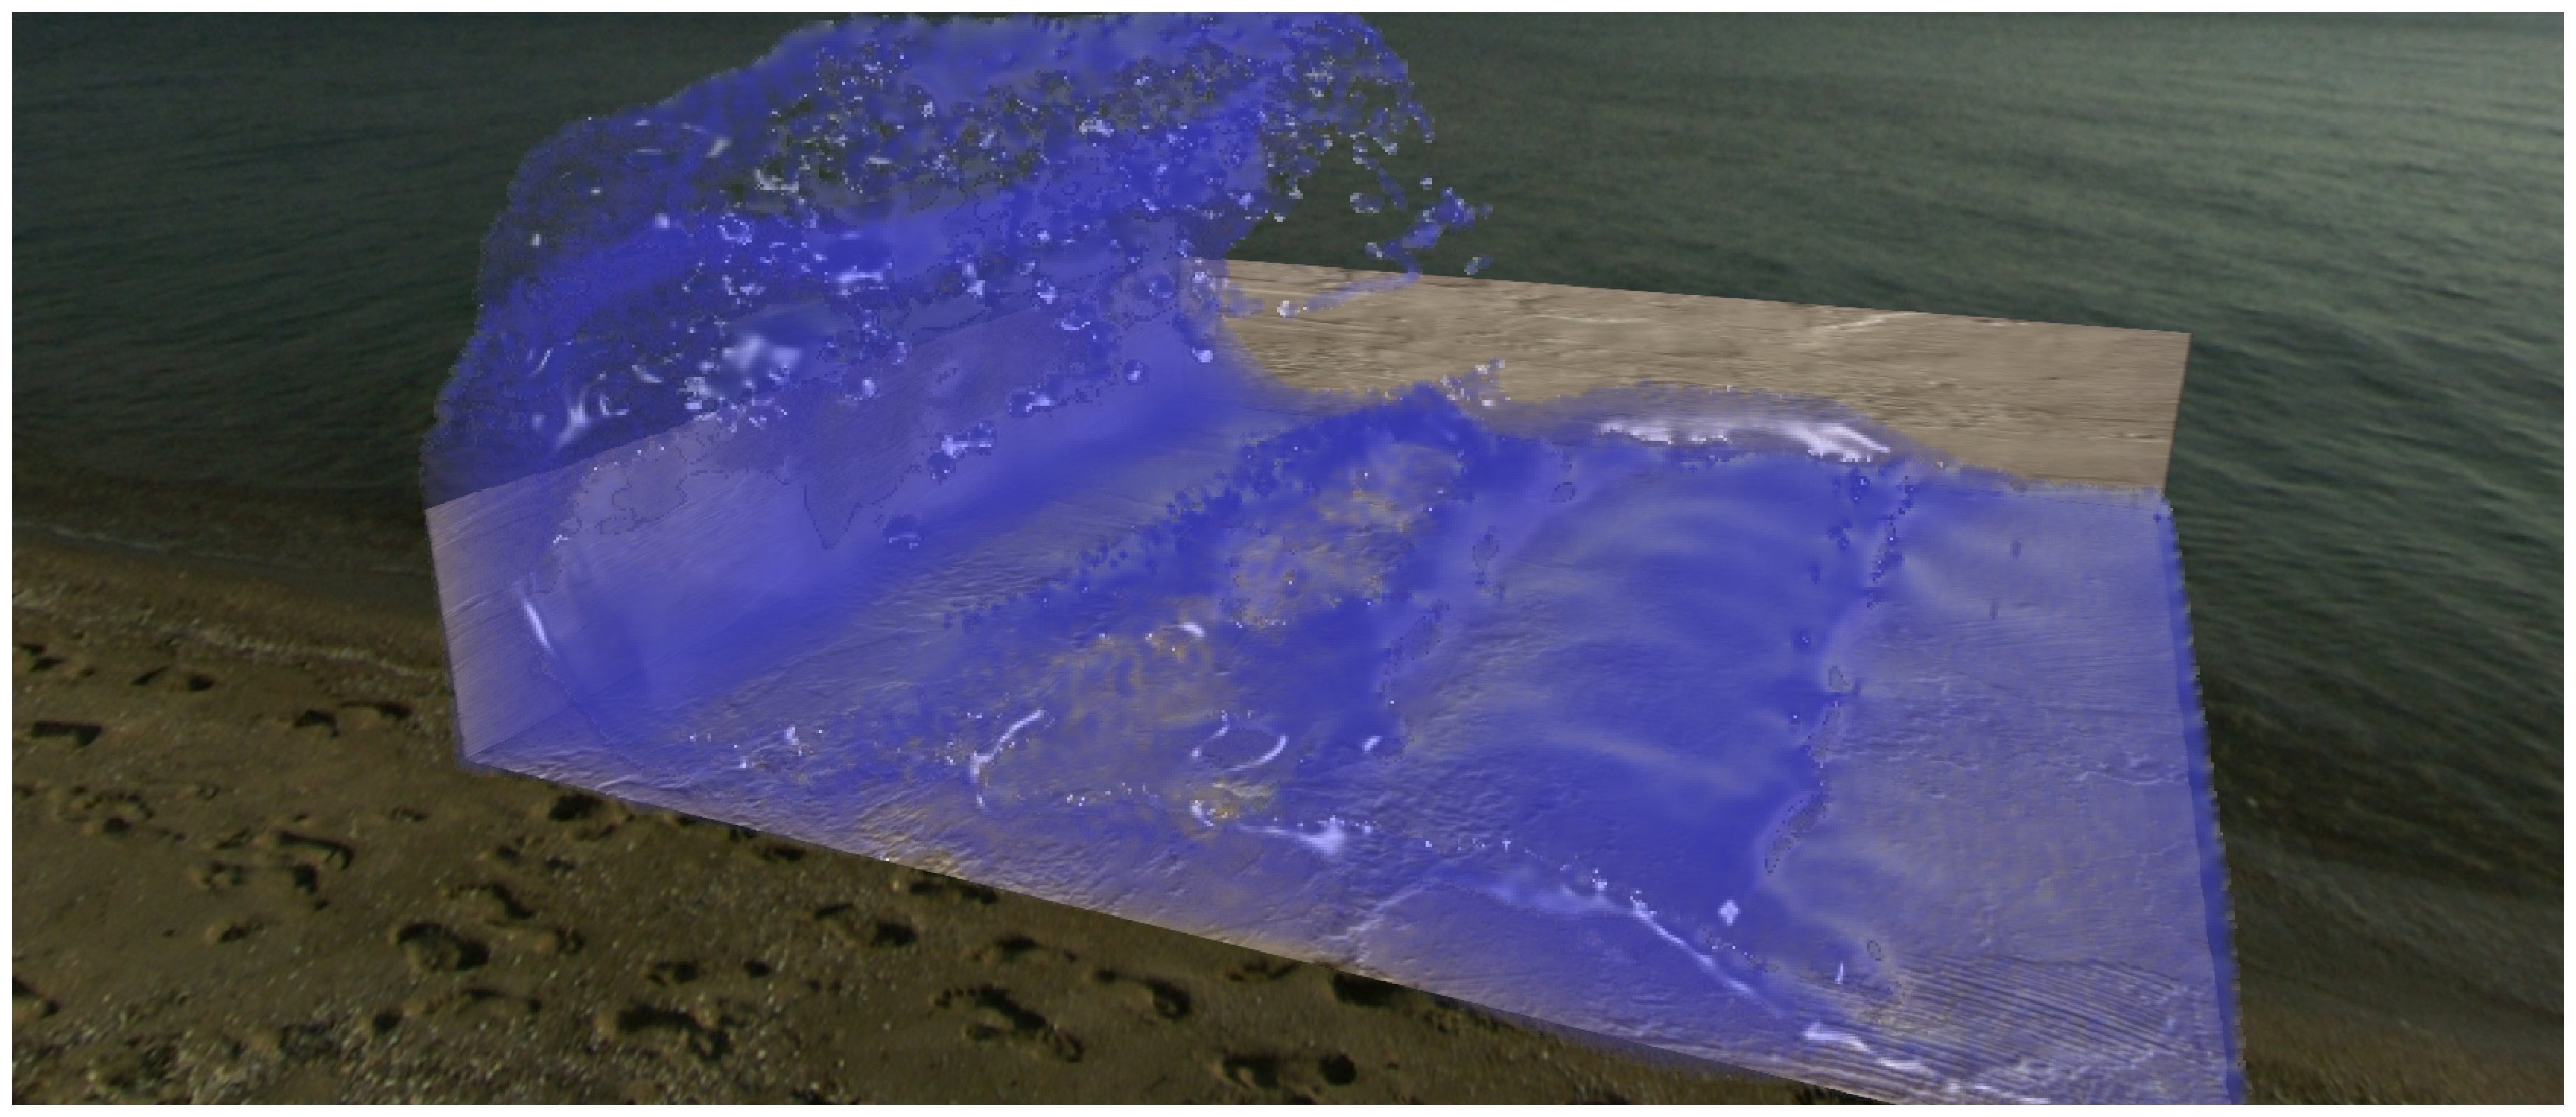
\includegraphics[height=2.5in]{images/teaser}
 \caption{Imagem final gerada utilizando 128K partículas de uma simulação SPH}
 }

\maketitle

\begin{abstract}

Este documento descreve a implementação do algoritmo IDW utilizando CUDA. Foram feitas 3 implementações do mesmo algoritmo: Uma em CPU; uma estratégia simples em CUDA utilizando somente memória global; e a última também em CUDA utilizando memória compartilhada e uma estratégia de \textit{tiling}. Foram feitos experimentos para comparar o tempo de execução entre os algoritmos e foi atingido um speedup de até xxx para os casos de teste.

\end{abstract}

\keywordlist

%% Use this only if you're preparing a technical paper to be published in the 
%% ACM 'Transactions on Graphics' journal.

%\TOGlinkslist

%% Required for all content. 

\copyrightspace

\section{Introdução}
A interpolação espacial é um método fundamental em geociencias, onde um número de dados conhecidos, como alturas de terreno por exemplo, são utilizados para predizer dados desconhecidos no mesmo modelo. O custo computacional destes algoritmos crescem de acordo com os dados de entrada conhecidos da interpolação e o número de dados que necessitam ser computados. Geralmente implementações seriais destes algoritmos se tornam muito custosas em relação ao tempo quando a quantidade de dados é grande.

O IDW, é o algoritmo mais comumente utilizado em interpolações espaciais, dado sua implementação bem simples e direta. Shepard, propôs uma função para a interpolação IDW bi-dimensional e é comumente utilizada. No método de Shepard, todos os valores conhecidos são utilizados para computar um valor interpolado, e cada cálculo por sua vez é independente de todos os outros, e, portanto, é facilmente paralelizável.

O advento da programação em placas gráficas nas últimas décadas, promoveu uma chamada natual para  que pesquisadores desenvolvessem soluções para problemas conhecidos em paralelo. O CUDA (Compute Unified Device Architeture), é uma plataforma para programação em paralelo e um modelo de programação criado pela NVIDIA, que permite explorar o poder de multiprocessamento de GPU's para solucionar problemas computationais complexos.

Neste trabalho foram desenvolvidas 3 versões do algoritmo IDW: uma sequencial em CPU, para fins de controle do tempo de de resposta em algoritmo; Uma versão simples em GPU, para identificar os ganhos com o poder de paralelismo das placas gráficas; E outra versão em GPU explorando o cache manual dos dados de entrada em memória shared visando diminuir o acesso à memória global da GPU que é conhecida por ser lenta.


\section{Metodologia}
Neste trabalho foi utilizado o método de Shepard simples para o cálculo da interpolação. O cálculo pode ser definido como: Seja $z_i$ o valor conhecido no ponto $D_i$, para calcular o ponto interpolado $P$ utilizamos a função de interpolação
\begin{equation}
f(P)=\left\{\begin{matrix}
\frac{\sum_{i=1}^{N}w_iz_i}{\sum_{i=1}^{N}w_i}, se\ d_i\neq 0
\\
z_i,\ se\ algum\ d_i = 0\ 

\end{matrix}\right.
\end{equation}

onde $w_i = d(P, D_i)^{-u}$ sendo $d$ uma métrica de distância, $u$ uma expoente definido pelo usuário.



\section{Resultados e discussões}


\section{Conclusão e trabalhos futuros}


\bibliographystyle{acmsiggraph}
\bibliography{template}
\end{document}
